\documentclass{../pl-slide}

\usepackage[british]{babel}
\usepackage[british]{datetime2}
\usepackage{amsmath}
\usepackage{amssymb}
\usepackage{ulem}
\usepackage{qrcode}

\usepackage{tikz,calc}
\usetikzlibrary{shapes, shapes, arrows, chains, fit, quotes}

\tikzstyle{trienode} = [draw=text-color, rounded corners]
\tikzstyle{bucket} = [draw=text-color, rectangle]

\definecolor{verystable}{HTML}{13f6e9}
\definecolor{stableenough}{HTML}{ccff00}
\definecolor{unstable}{HTML}{ffa500}

\settheme{ipfs-thing-2023}

%Information to be included in the title page:
\title{Composable DHT}
\subtitle{Enabling More Applications to Join the libp2p DHT Ecosystem}
\author{Gui Michel}
\avatar{../resources/avatar.jpg}
\handle{@guissou}
\group{Probelab}
\institute{Protocol Labs}
\event{IPFS Thing}
\date{\DTMdate{2023-04-15}}

\begin{document}

\frame{\titlepage}

\begin{frame}
\frametitle{Disclaimer}

\begin{columns}[onlytextwidth]
	\begin{column}{0.59\textwidth}
		\begin{itemize}
			\itemc Very early design prototype
			\itemc Gather communuity feedback
		\end{itemize}
	\end{column}
		\begin{column}{0.39\textwidth}
    		\begin{center}
        		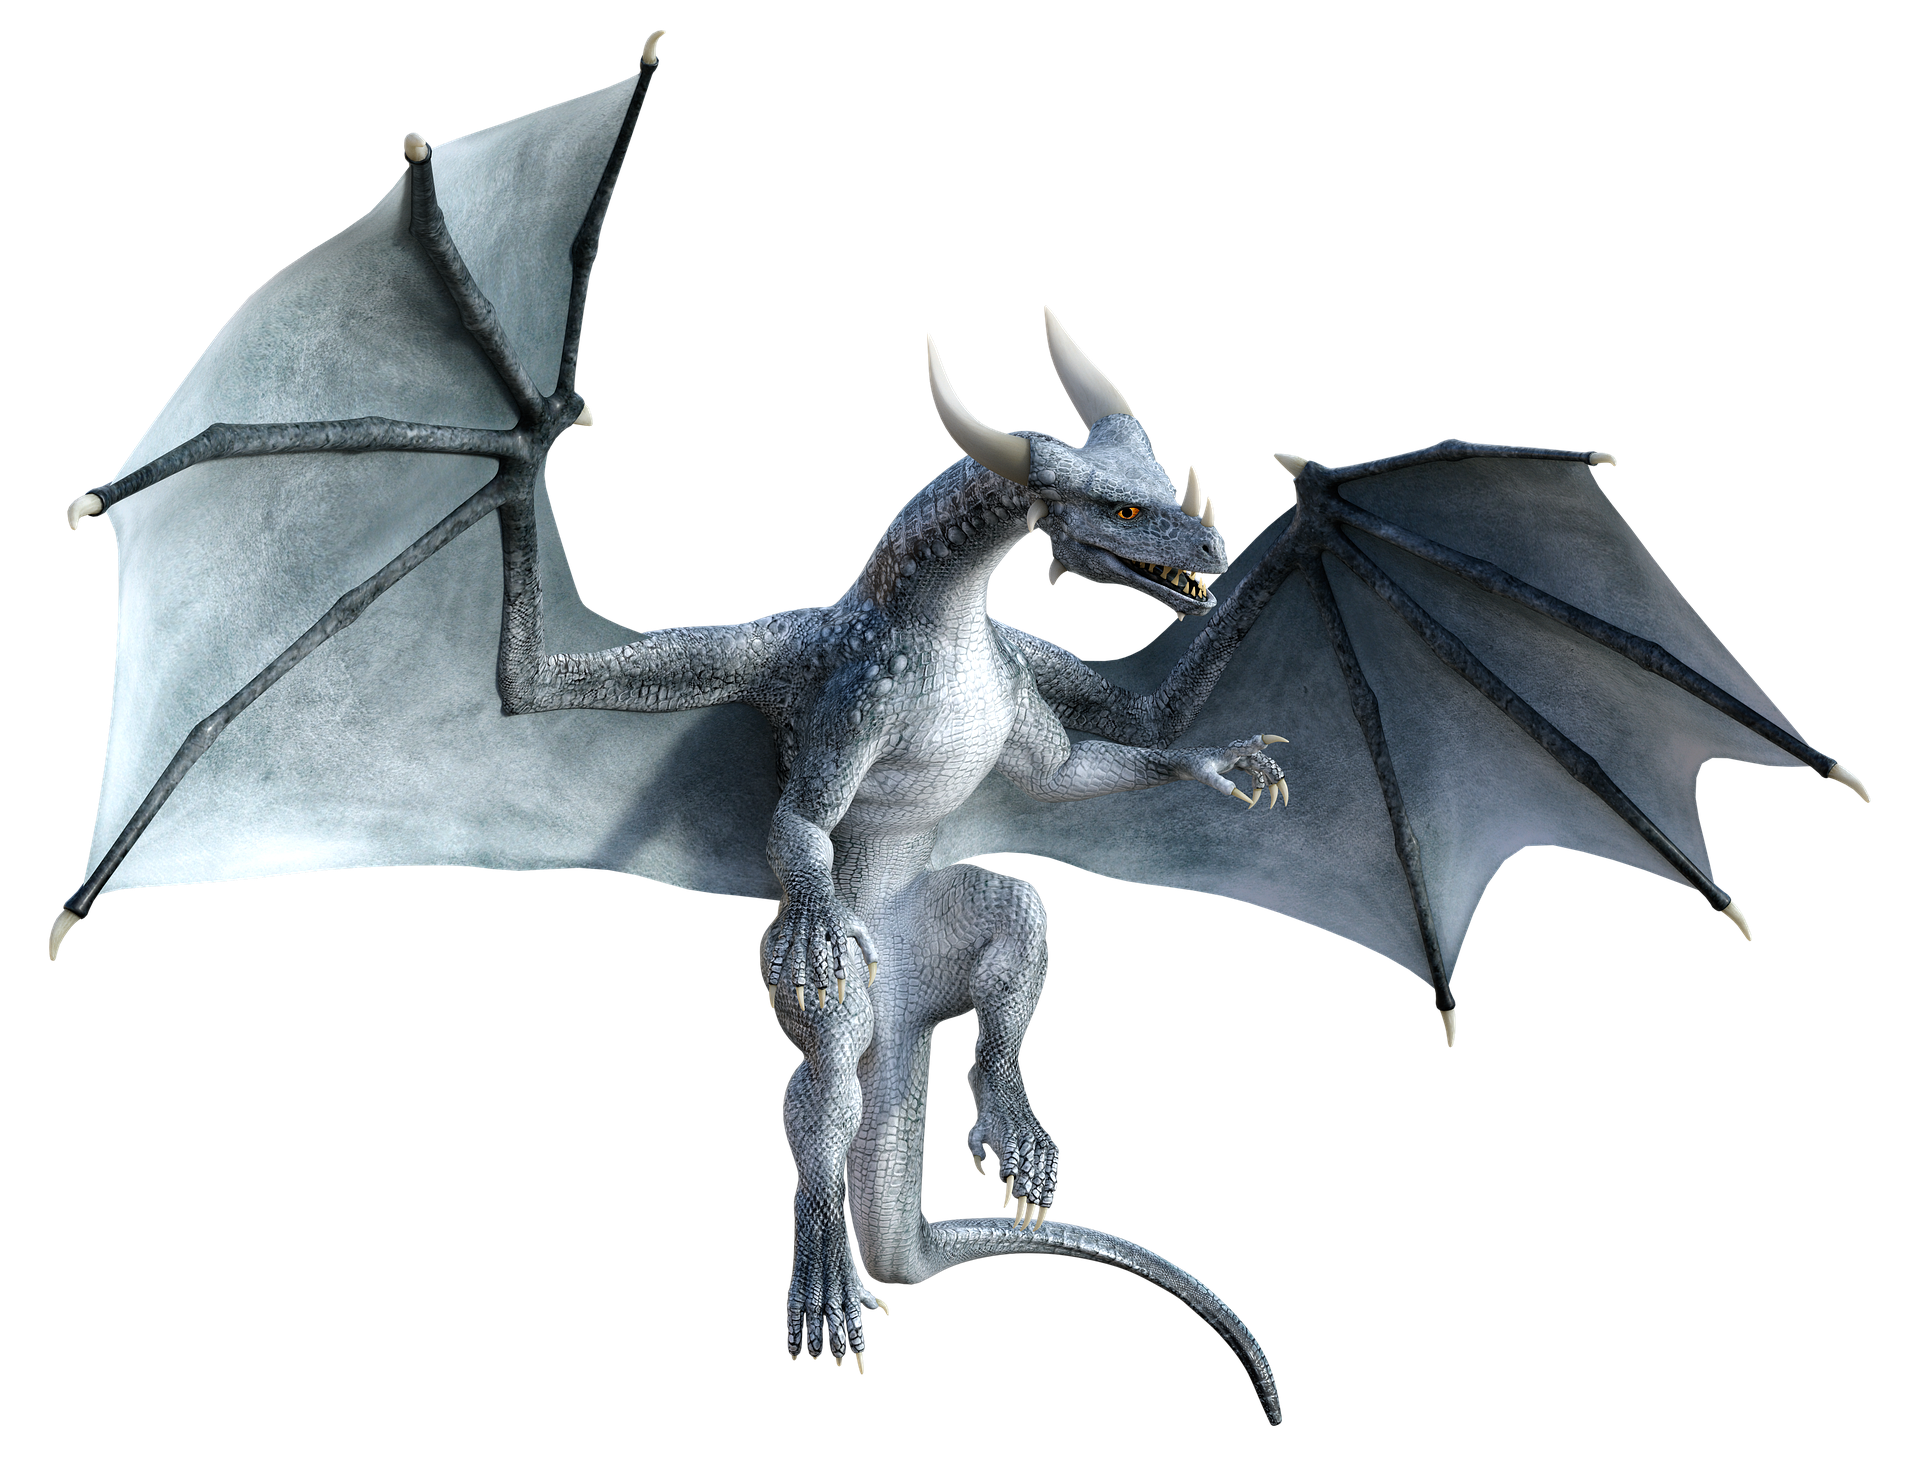
\includegraphics[width=13em]{resources/dragon.png}
        		\textit{Here be dragons}
    		\end{center}
	\end{column}

\end{columns}
\end{frame}


\begin{frame}
\frametitle{Kademlia DHT}

\begin{columns}[onlytextwidth]
	\begin{column}{0.64\textwidth}
		\begin{itemize}
			\itemc A Distributed Hash Table (DHT) is a decentralized overlay network used for peer and content routing
			\itemc Each node is uniquely identified by a binary \texttt{Key}, determining the node's position in the Keyspace and the distance between nodes
			\itemc Routing table groups nodes into \textit{buckets} based on their distance from the local node's \texttt{Key}, bucket \texttt{i} containing peers \texttt{ID} sharing a \texttt{i} bit prefix
			\itemc Iterative lookups to efficiently find peers and content in the network, making it highly scalable
		\end{itemize}
	\end{column}
		\begin{column}{0.34\textwidth}
    		\begin{center}
        		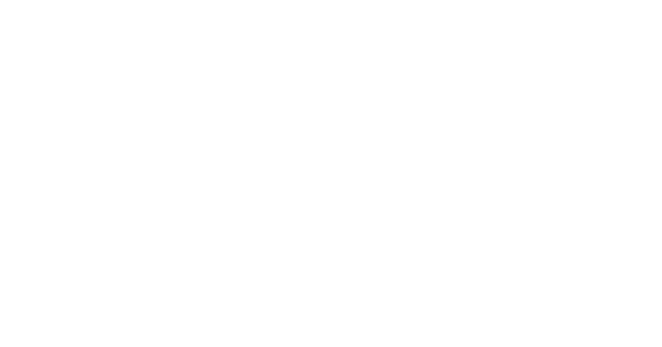
\includegraphics[width=13em]{resources/kademlia-trie.png}
        		\textit{Kademlia Binary Trie}
    		\end{center}
	\end{column}

\end{columns}
\end{frame}

\begin{frame}
\frametitle{Libp2p Kademlia DHT Protocol}

\begin{itemize}
	\itemc IPFS-centric Kademlia implementations
	\itemc Kad DHT is the peer routing component of Libp2p
	\itemc Not future proof
	\bigskip
	\item[\greencube] The implementations are correct but the protocol is flawed
\end{itemize}
\end{frame}

\begin{frame}
\frametitle{Building a P2P messaging app using Libp2p}

\begin{itemize}
	\itemc Routing and Hole Punching using the DHT as  peer discovery mechanism 
	\itemc Feature: Rendez-vous for group chats	
	\itemc Don't want nodes to store and serve IPFS data
	\itemc If participating in the DHT but not serving IPFS data, IPFS will be hurt
	\bigskip
	\item[\greencube] Other apps cannot really use the Libp2p DHT, they have to implement their own
\end{itemize}
\end{frame}

\begin{frame}
\frametitle{Current DHT stack}
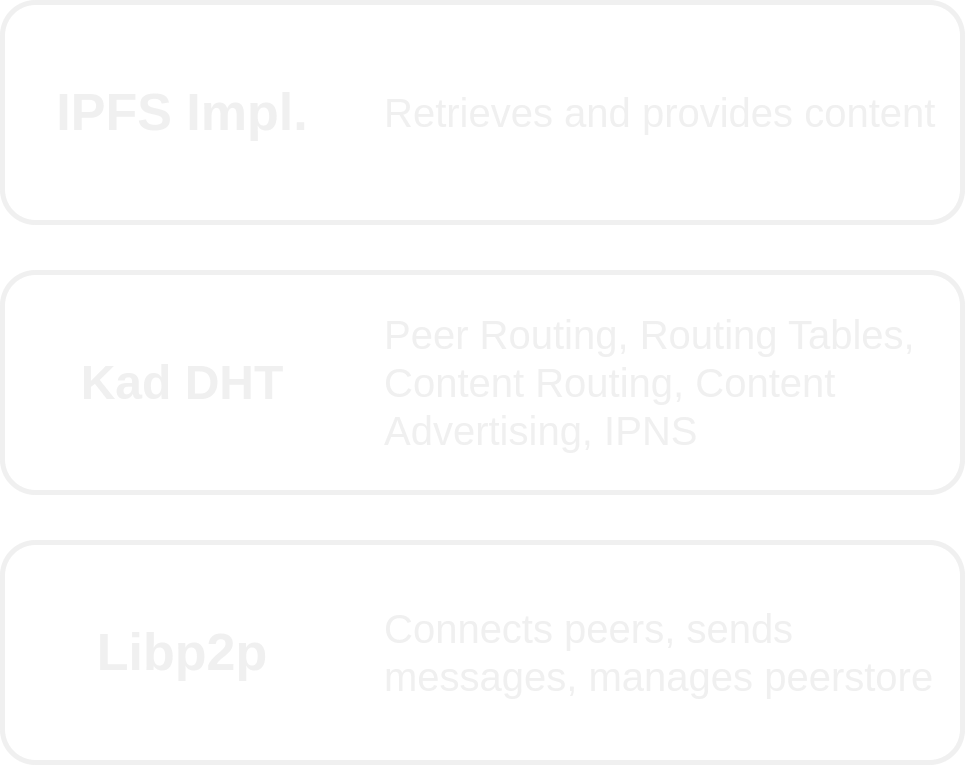
\includegraphics[scale=.2]{resources/old-dht-stack.png}
\end{frame}

\begin{frame}
\frametitle{Current DHT stack}
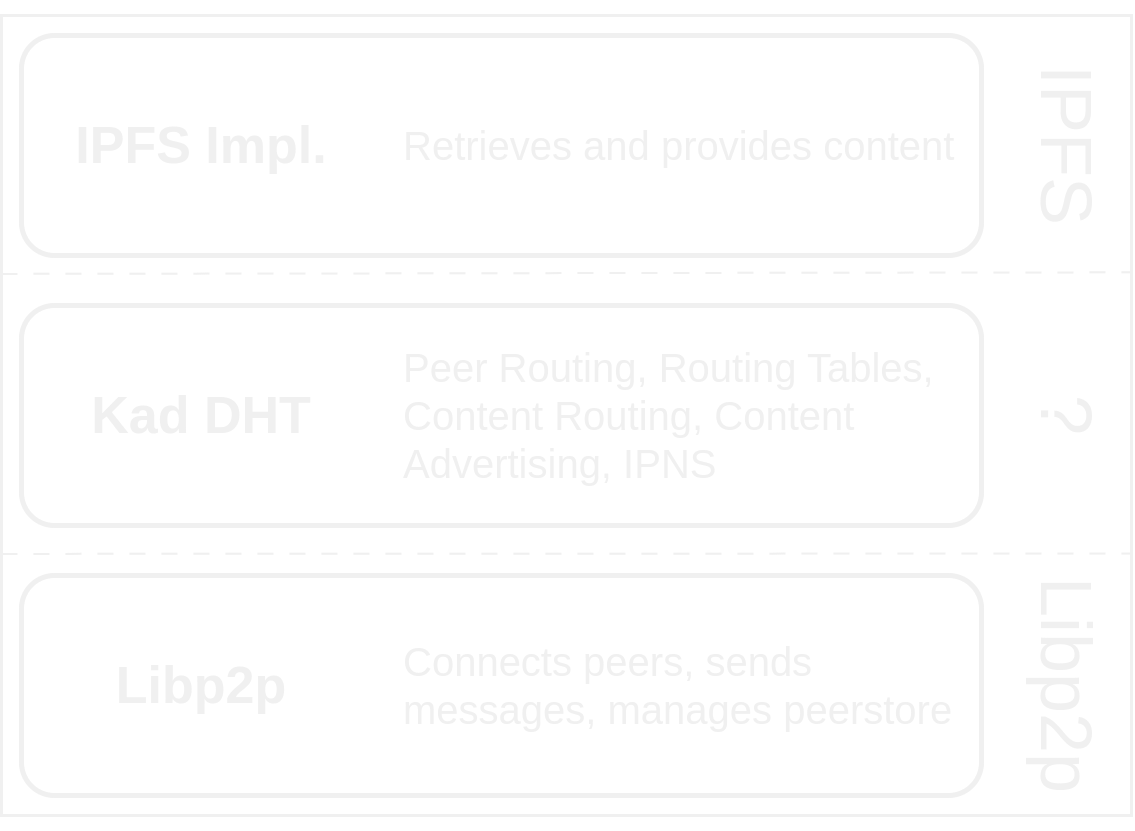
\includegraphics[scale=.2]{resources/old-dht-stack-cat.png}
\end{frame}

\begin{frame}
\frametitle{Improved DHT stack}
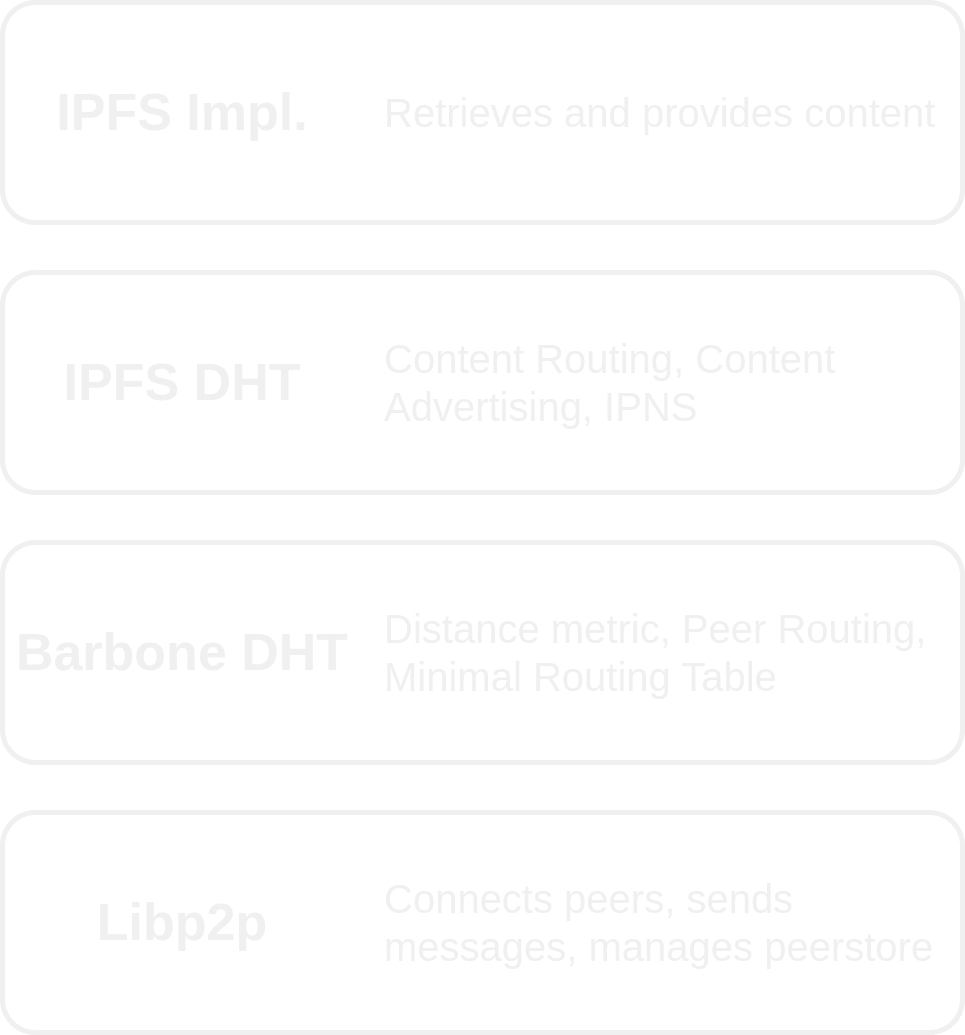
\includegraphics[scale=.18]{resources/improved-dht-stack.png}
\end{frame}
\begin{frame}
\frametitle{Improved DHT stack}
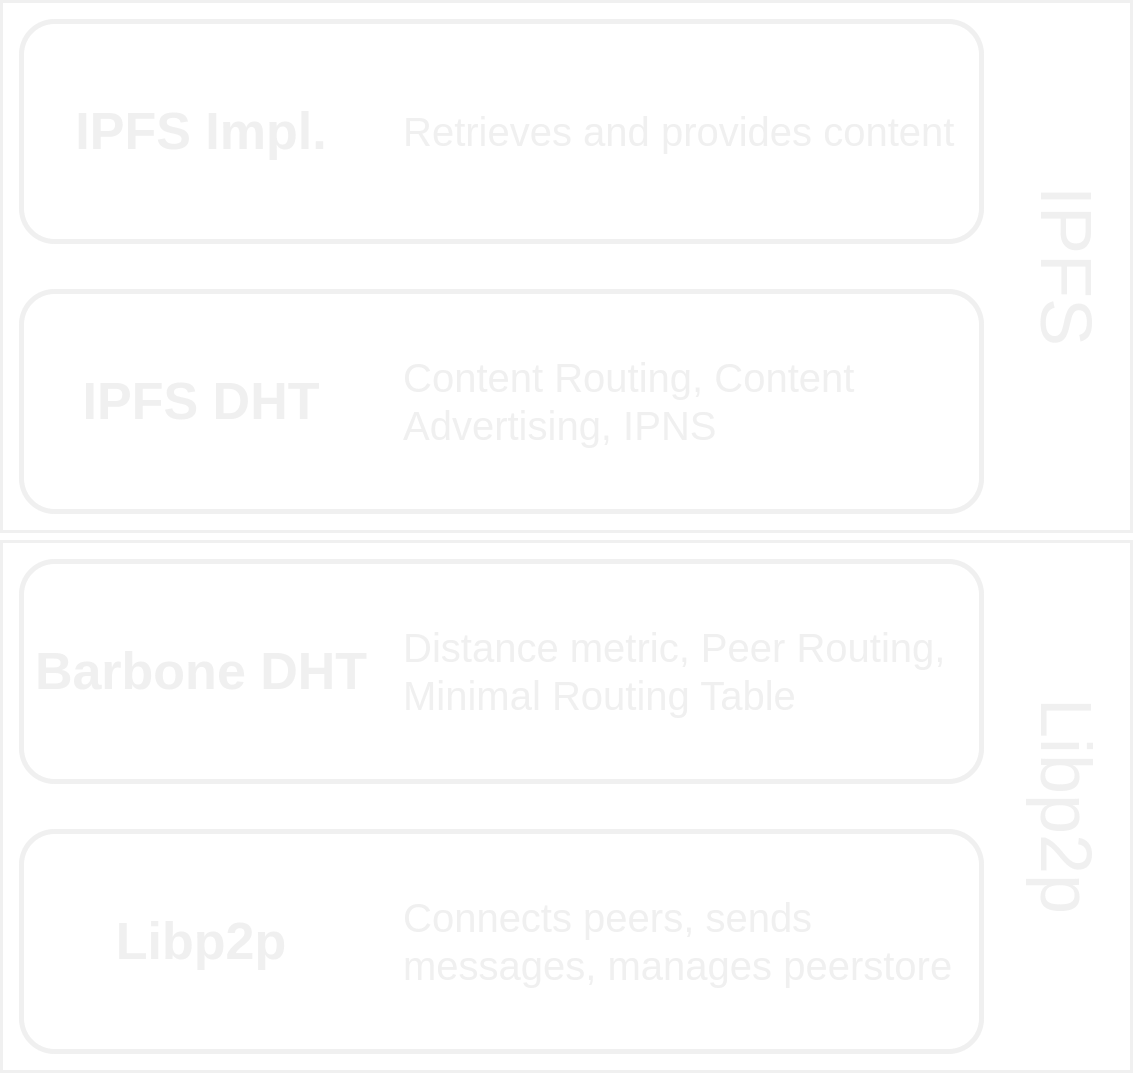
\includegraphics[scale=.18]{resources/improved-dht-stack-cat.png}
\end{frame}

\begin{frame}
\frametitle{Improved DHT stack}
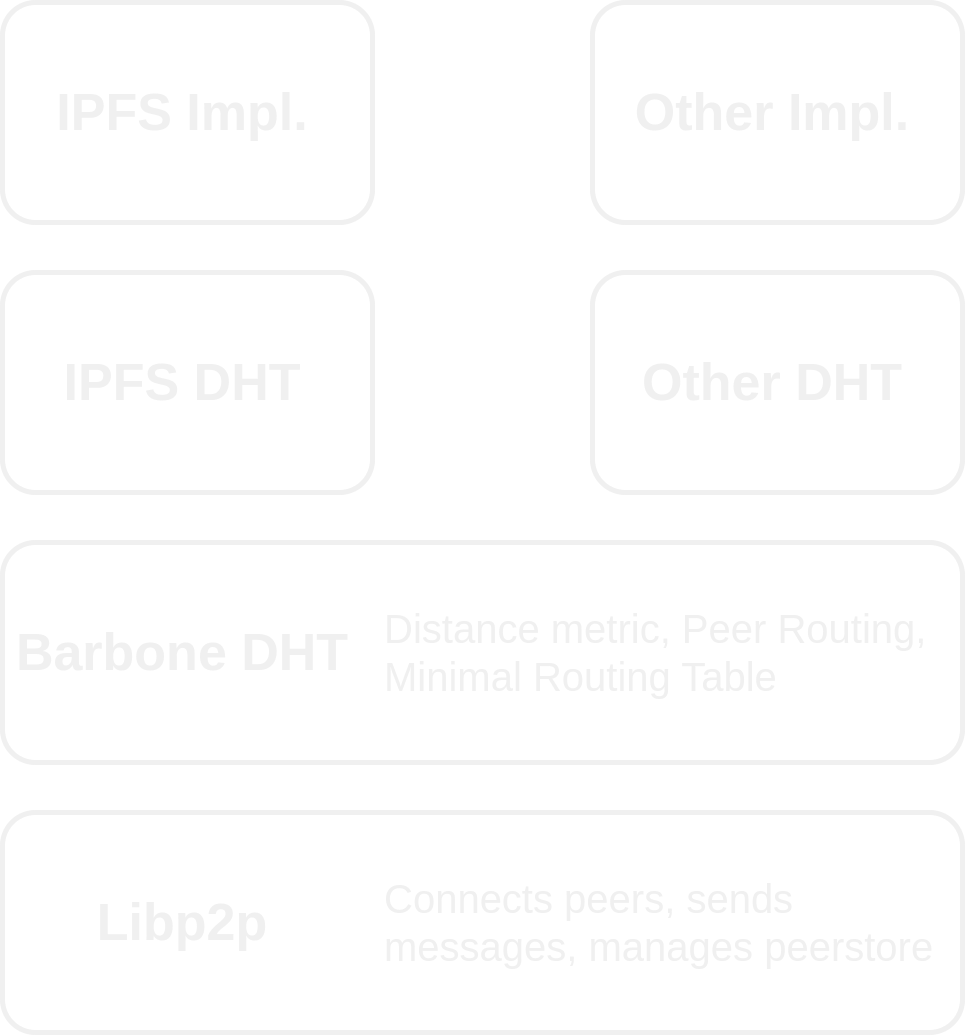
\includegraphics[scale=.18]{resources/improved-dht-mult-stack.png}
\end{frame}
\begin{frame}
\frametitle{Improved DHT stack}
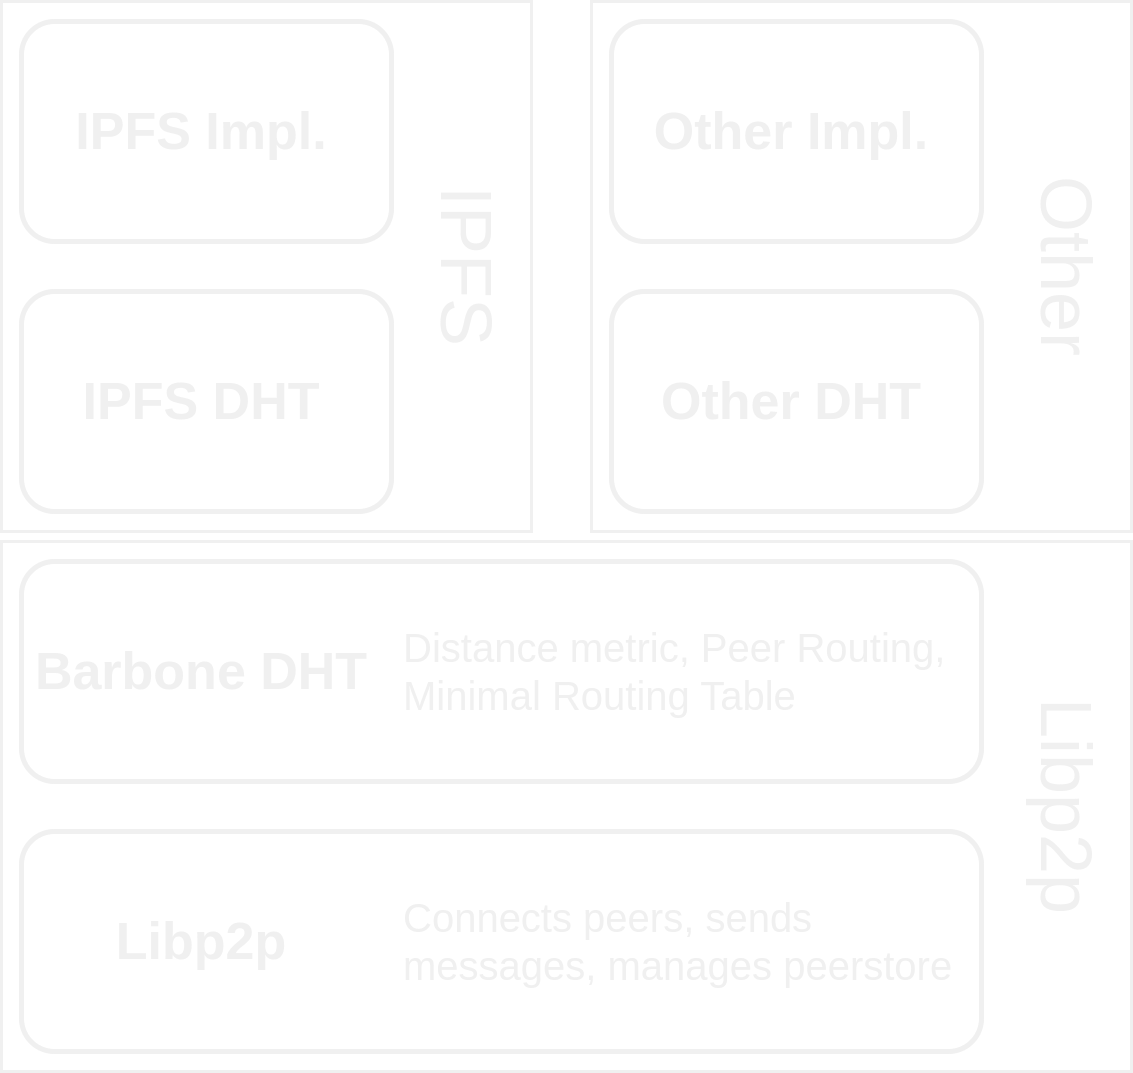
\includegraphics[scale=.18]{resources/improved-dht-mult-stack-cat.png}
\end{frame}

\begin{frame}
\frametitle{But wait, it doesn't work!}
\begin{columns}
	\begin{column}{0.49\textwidth}
	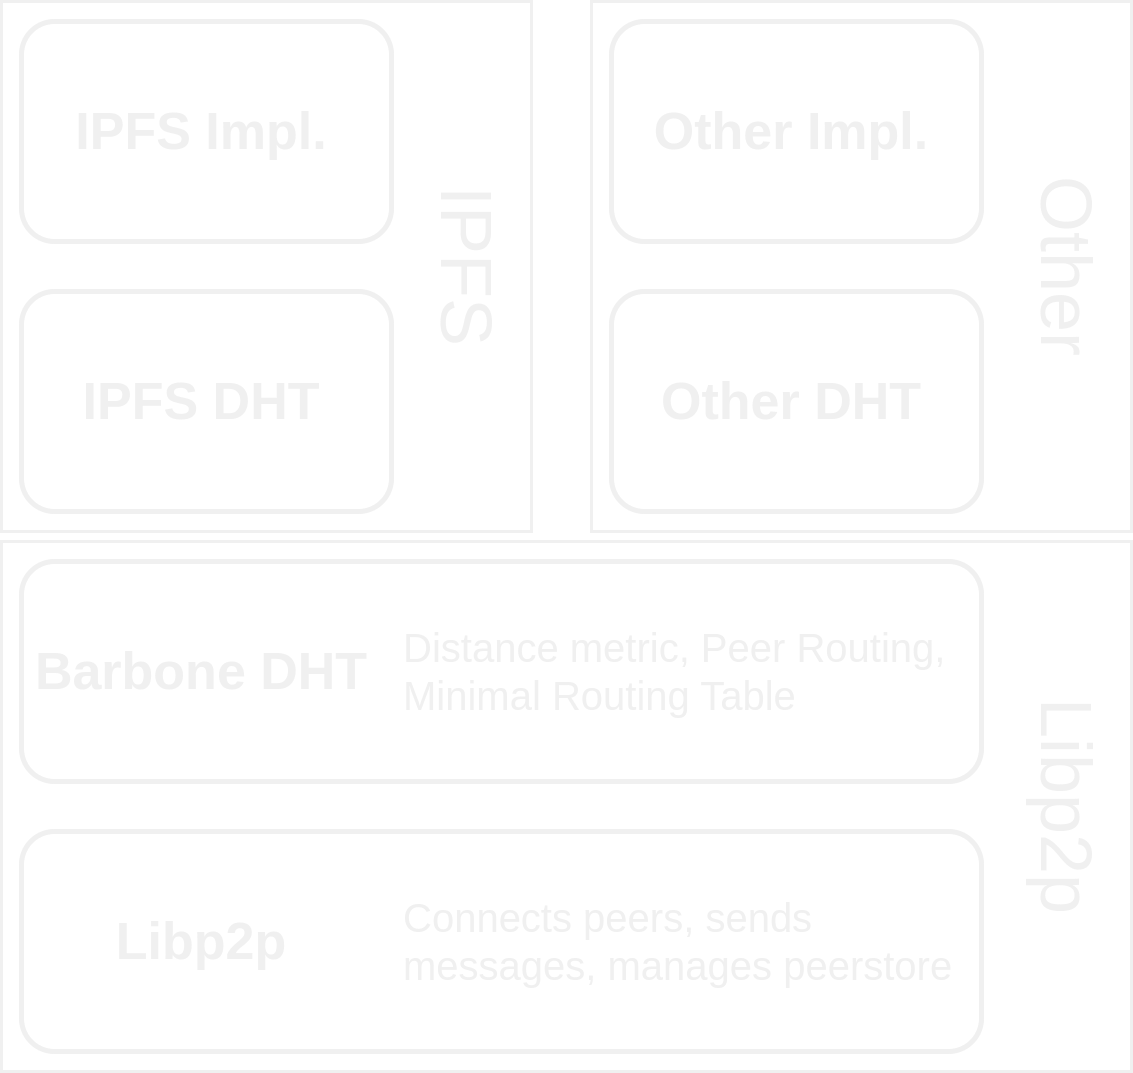
\includegraphics[scale=.18]{resources/improved-dht-mult-stack-cat.png}
	\end{column}
		\begin{column}{0.49\textwidth}
        		\begin{itemize}
        			\itemc IPFS \texttt{Provide} won't exactly work
        			\itemc IPFS \texttt{FindProvs} will not be accurate
        			\bigskip
        			\item[\greencube] Unless we change the \texttt{IPFS DHT} Protocol!
        		\end{itemize}
	\end{column}

\end{columns}
\end{frame}

\begin{frame}
\frametitle{Adapting the IPFS DHT Protocol}
\begin{columns}
	\begin{column}{0.49\textwidth}
	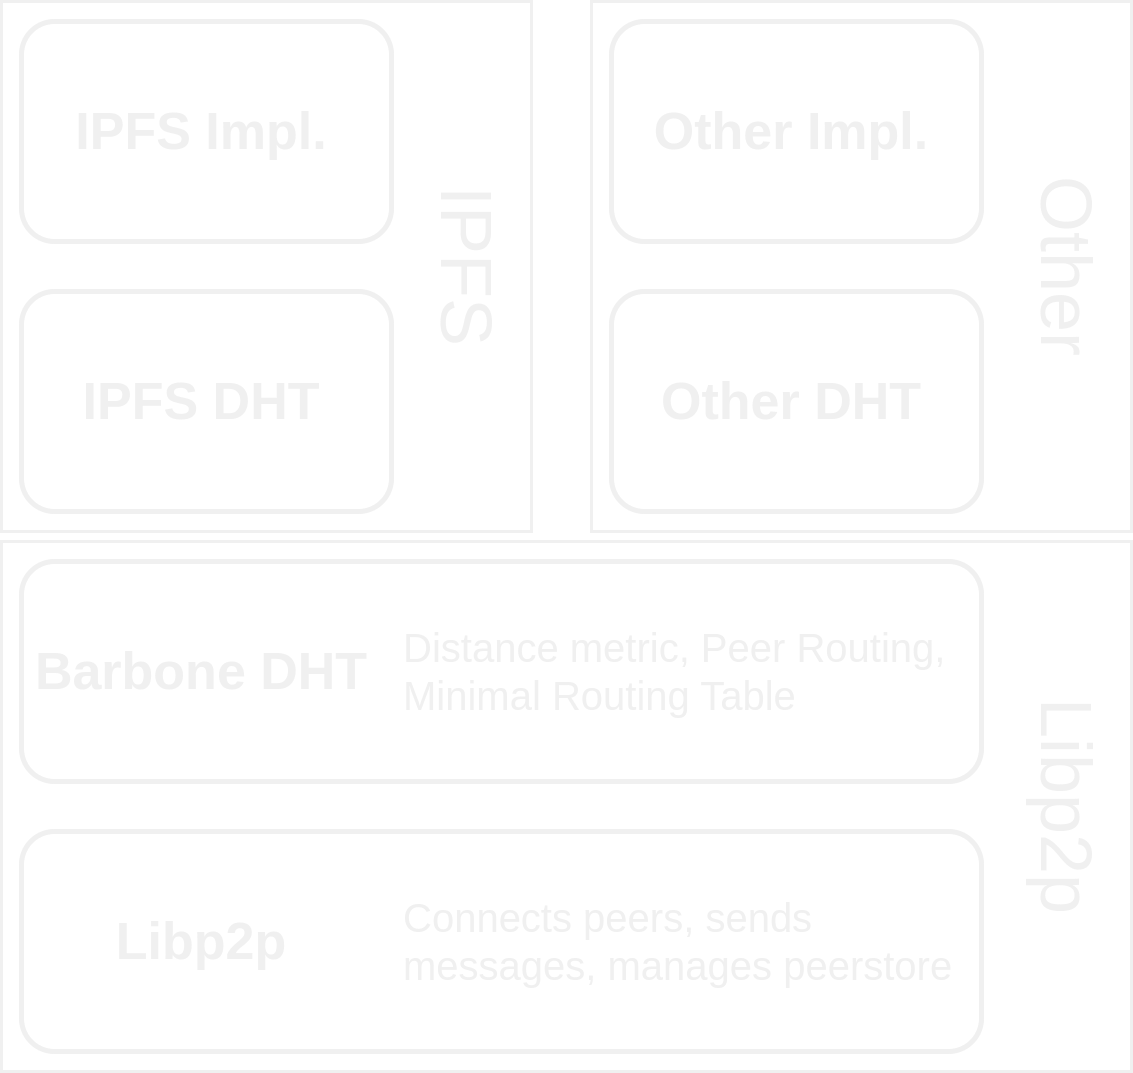
\includegraphics[scale=.18]{resources/improved-dht-mult-stack-cat.png}
	\end{column}
		\begin{column}{0.49\textwidth}
        		\begin{itemize}
				\itemc IPFS content should be allocated to IPFS nodes only
				\itemc IPFS content should be looked up on IPFS nodes only
				\itemc Same for Other DHT's RPCs
				\itemc Peer Routing still works like before
				\bigskip
				\item[\greencube] How do we segregate applications?
        		\end{itemize}
	\end{column}

\end{columns}
\end{frame}

\begin{frame}
\frametitle{Features \& Protocols}
\begin{itemize}
	\itemc A \textit{Feature} is defined as support for a specific RPC
	\itemc A \textit{Protocol} is defined as a set of features
	\itemc In a Protocol, Features must be ordered according to their importance
	\itemc Each node advertises its ordered set of features when communicating\\with a remote peer
	\itemc The features are recorded in the Routing Table for each remote peer
\end{itemize}
\end{frame}

\begin{frame}
\frametitle{Routing Table Peer Selection Process}
\begin{itemize}
	\itemc Currently based on seniority only
	\bigskip
	\item[\greencube] New selection criteria
	\begin{enumerate}
		\item Features preferences
		\item Seniority
	\end{enumerate}
\end{itemize}
\end{frame}

\begin{frame}
\frametitle{Routing Table Peer Selection Example}
\begin{center}
	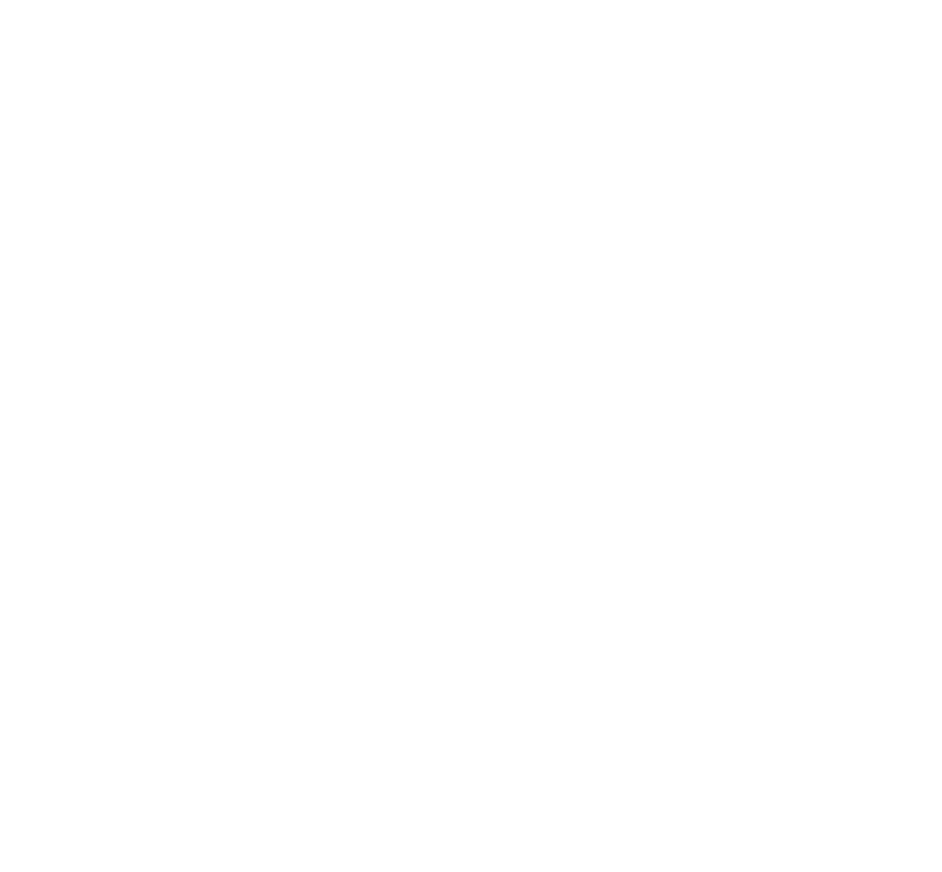
\includegraphics[scale=.23]{resources/trie-vanilla.png}
\end{center}
\end{frame}

\begin{frame}
\frametitle{Routing Table Peer Selection Example}
\begin{center}
	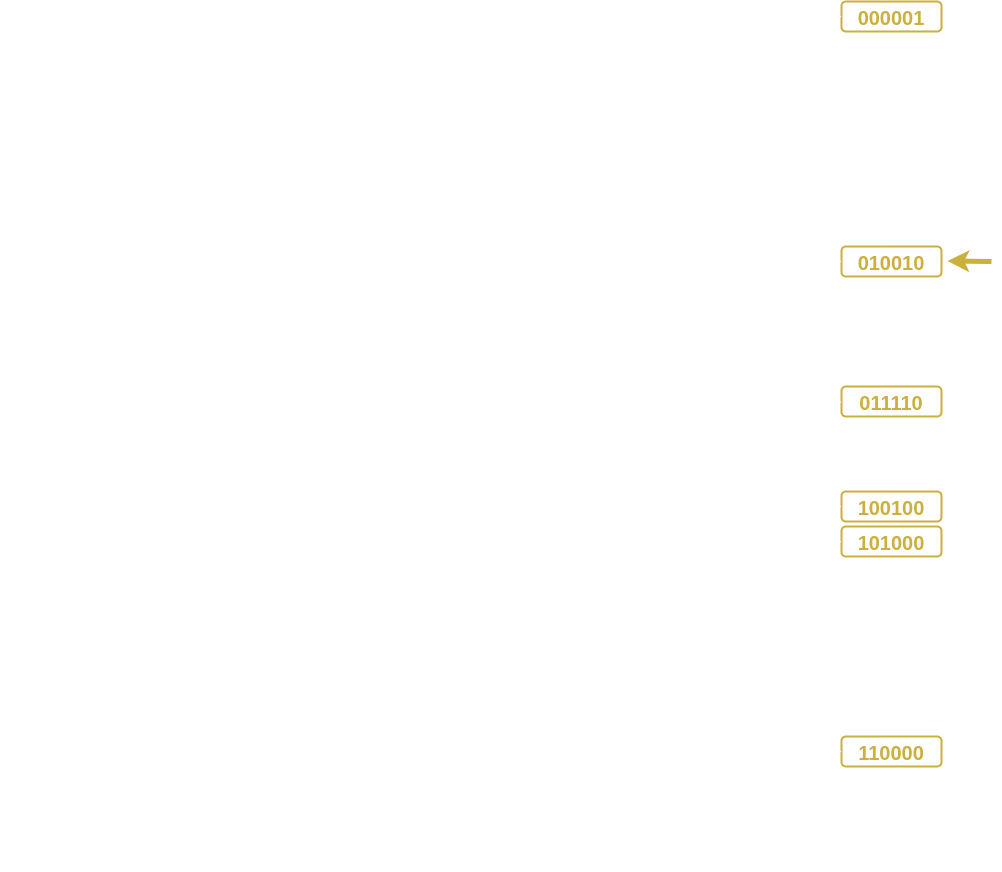
\includegraphics[scale=.23]{resources/trie-features.png}
\end{center}
\end{frame}

\begin{frame}
\frametitle{Routing Table Peer Selection Example}
\begin{center}
	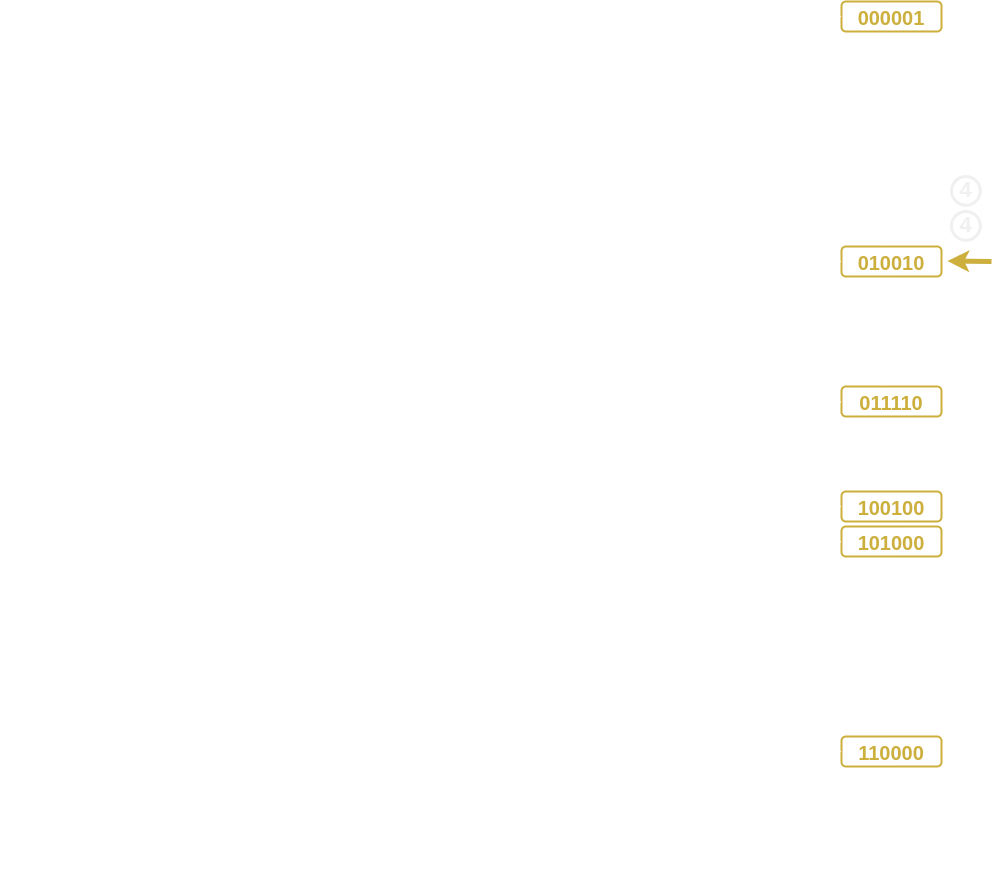
\includegraphics[scale=.23]{resources/trie-features-bucket4.png}
\end{center}
\end{frame}

\begin{frame}
\frametitle{Routing Table Peer Selection Example}
\begin{center}
	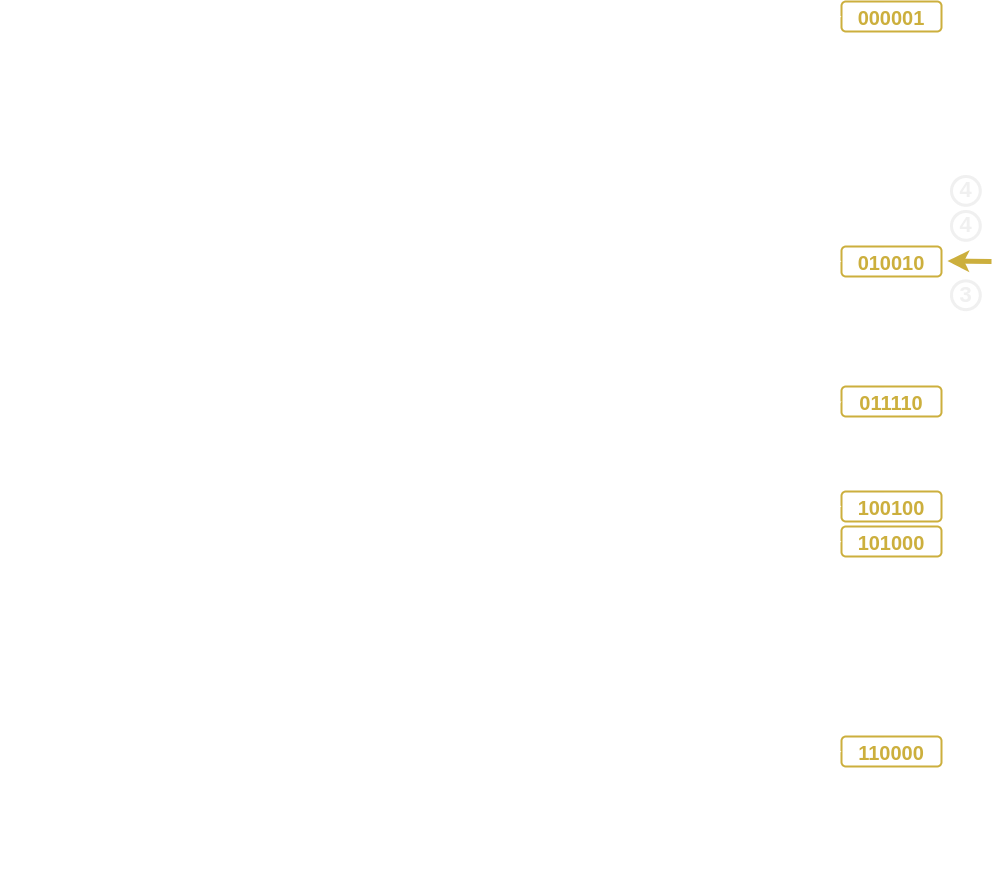
\includegraphics[scale=.23]{resources/trie-features-bucket3.png}
\end{center}
\end{frame}

\begin{frame}
\frametitle{Routing Table Peer Selection Example}
\begin{center}
	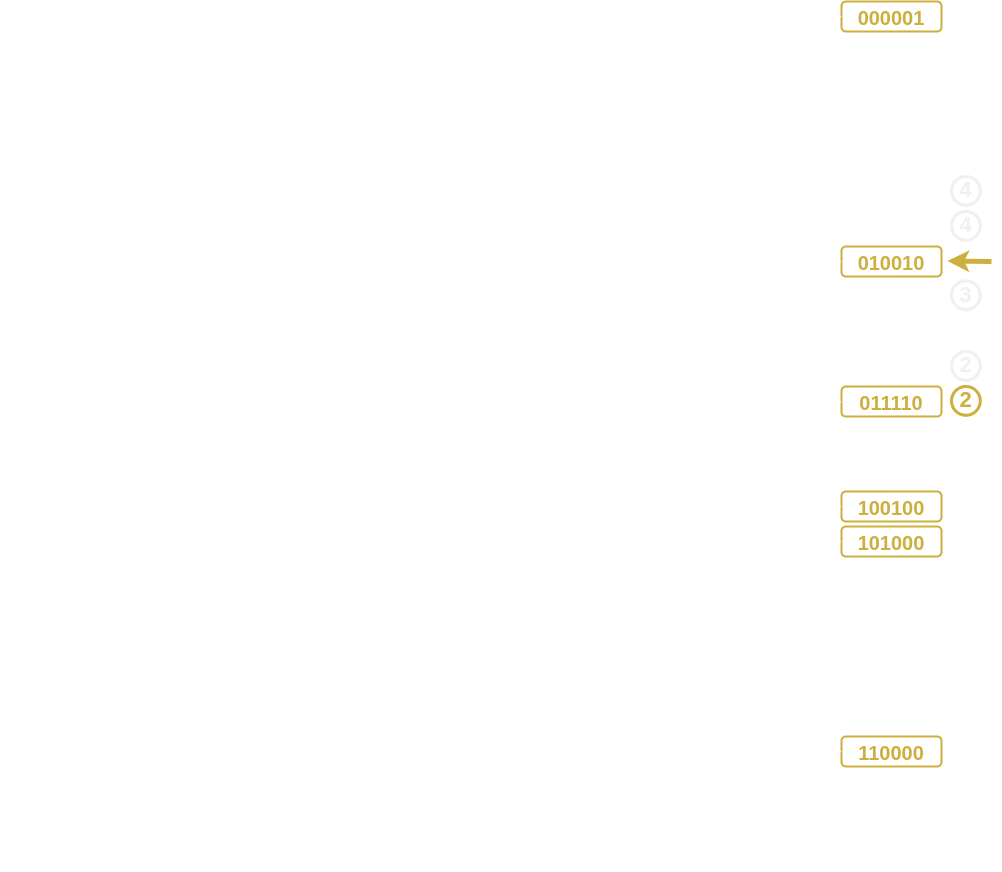
\includegraphics[scale=.23]{resources/trie-features-bucket2.png}
\end{center}
\end{frame}

\begin{frame}
\frametitle{Routing Table Peer Selection Example}
\begin{center}
	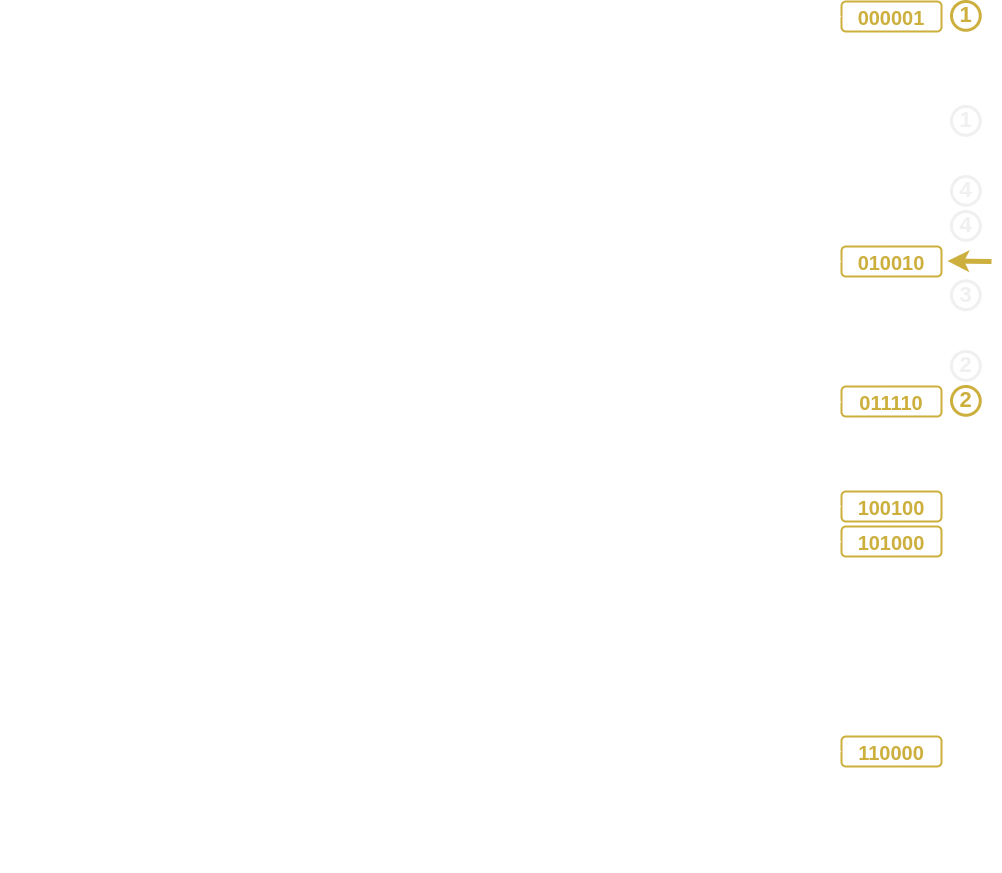
\includegraphics[scale=.23]{resources/trie-features-bucket1.png}
\end{center}
\end{frame}

\begin{frame}
\frametitle{Routing Table Peer Selection Example}
\begin{center}
	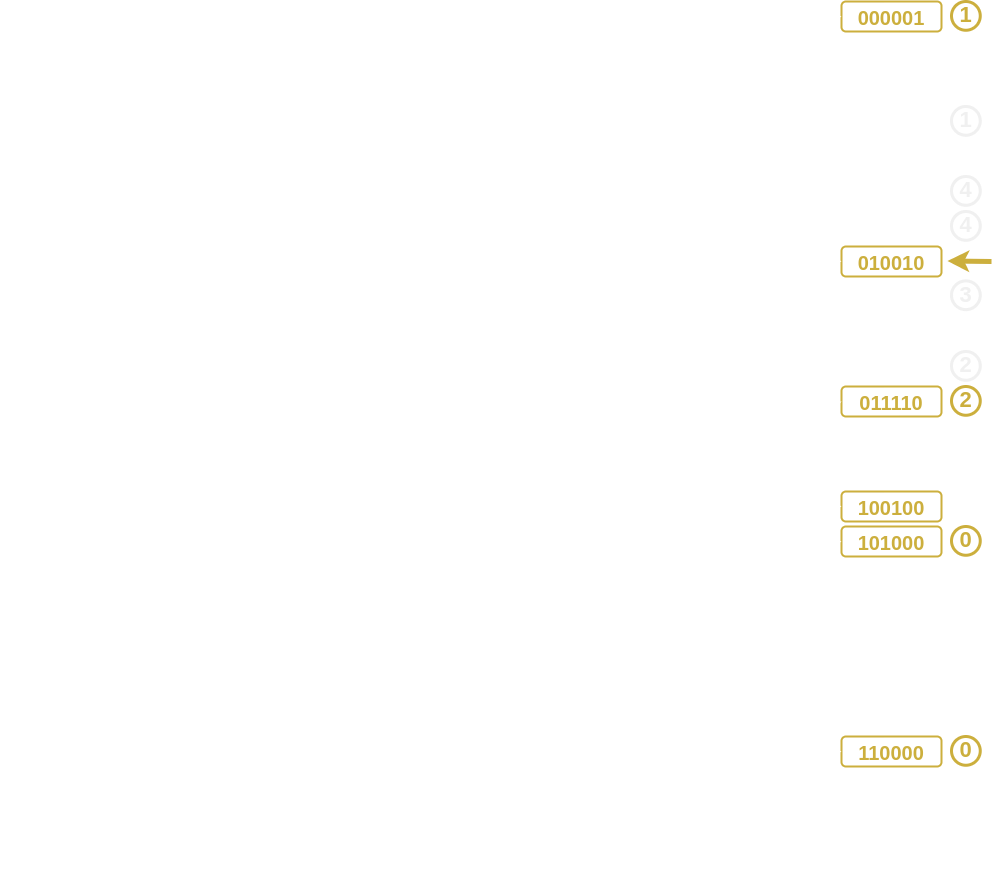
\includegraphics[scale=.23]{resources/trie-features-bucket0.png}
\end{center}
\end{frame}


\begin{frame}
\frametitle{Routing Table Peer Selection Example}
\begin{center}
	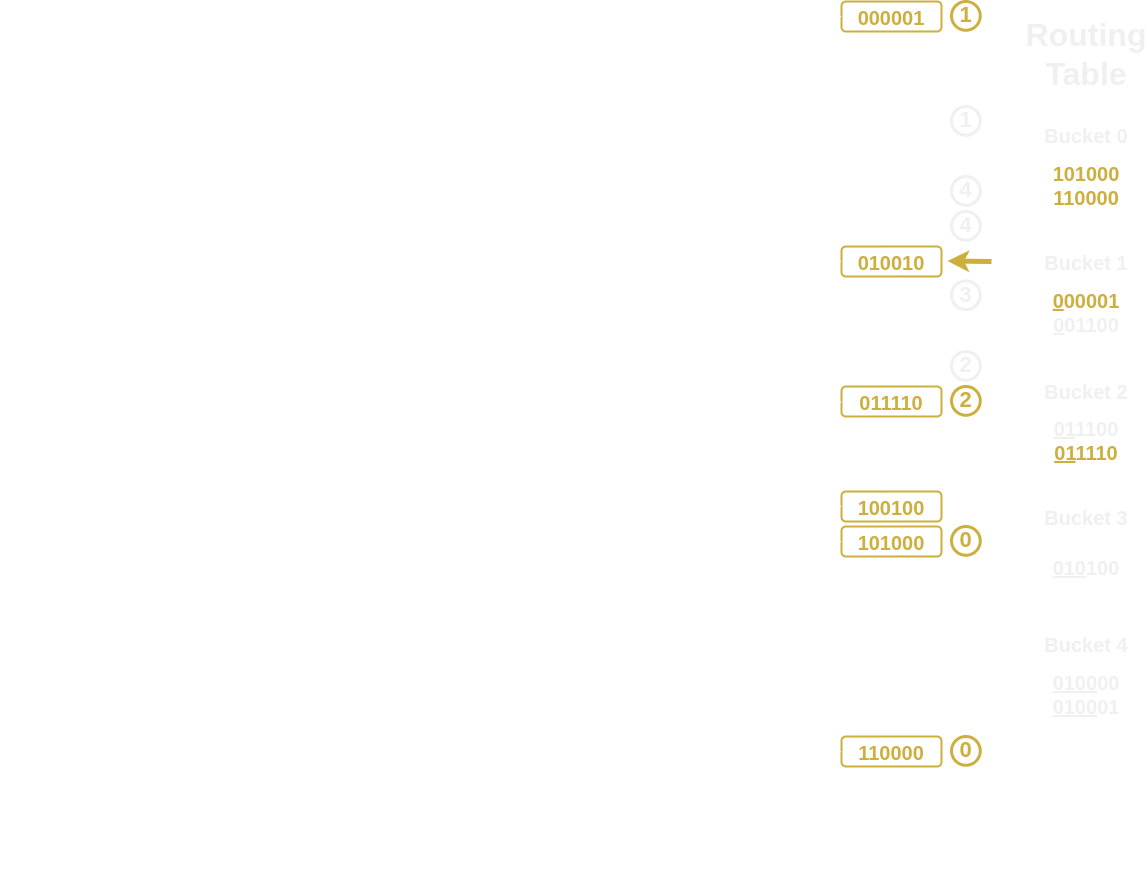
\includegraphics[scale=.23]{resources/trie-features-rt.png}
\end{center}
\end{frame}

\begin{frame}
\frametitle{Routing Table Peer Selection Example}
\begin{center}
	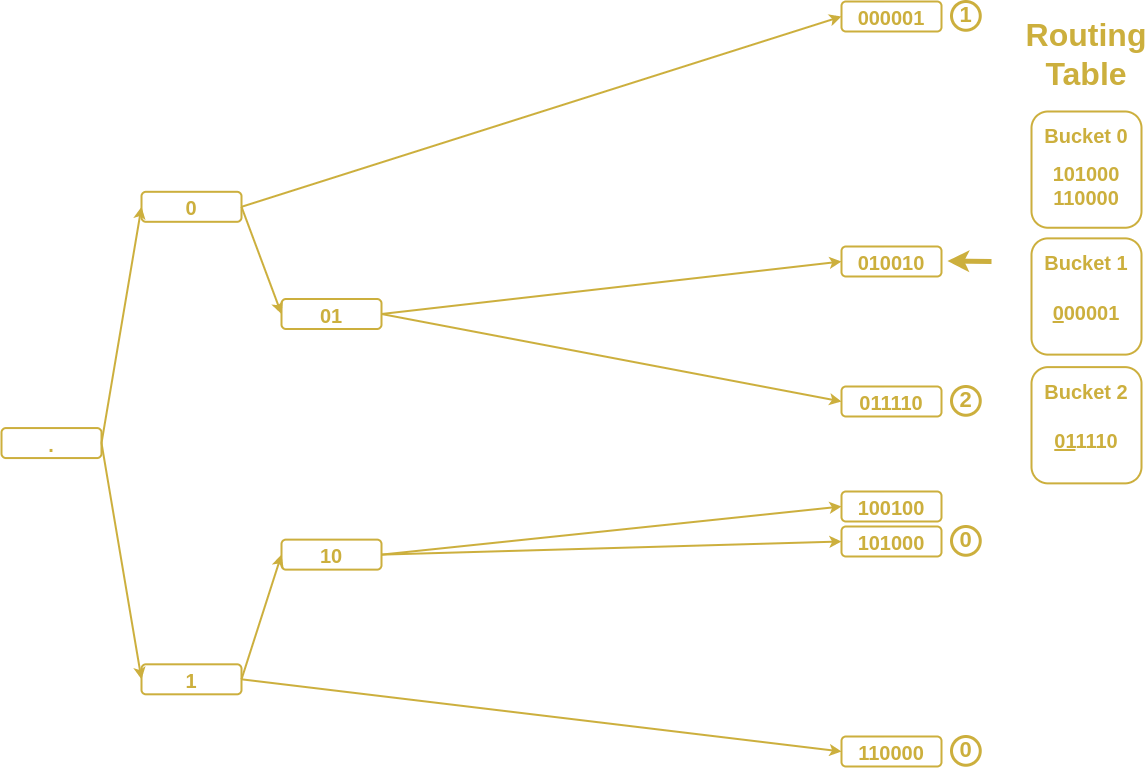
\includegraphics[scale=.23]{resources/trie-features-subdht.png}
\end{center}
\end{frame}

\begin{frame}
\frametitle{Query process}
\begin{itemize}
	\itemc In peer lookup, indicate your features priorities
	\itemc Requested peers return in priority peers matching the features priorities
	\itemc Requested peers' routing table is expected to have the same features
	\bigskip
	\item[\greencube] Feature specific RPC only stays in the feature's sub-DHT
\end{itemize}
\end{frame}

\begin{frame}
\frametitle{Routing Table Multi-Features Peers Selection}
\begin{columns}[onlytextwidth]
	\begin{column}{0.49\textwidth}
	    		\begin{center}
        		
\includegraphics[scale=.35]{resources/1-plan.png}\\
        		\medskip
        		\textit{Kademlia keyspace 2D\\distance projection}
        		\end{center}
	\end{column}
	\begin{column}{0.49\textwidth}
	\end{column}

\end{columns}
\end{frame}

\begin{frame}
\frametitle{Routing Table Multi-Features Peers Selection}
\begin{columns}[onlytextwidth]
	\begin{column}{0.49\textwidth}
	    		\begin{center}
        		
\includegraphics[scale=.35]{resources/1-plan-buckets.png}\\
        		\medskip
        		\textit{Kademlia keyspace 2D\\distance projection}
        		\end{center}
	\end{column}
	\begin{column}{0.49\textwidth}
	\end{column}

\end{columns}
\end{frame}



\begin{frame}
\frametitle{Routing Table Multi-Features Peers Selection}
\begin{columns}[onlytextwidth]
	\begin{column}{0.49\textwidth}
	    		\begin{center}
        		
\includegraphics[scale=.35]{resources/1-plan-buckets.png}\\
        		\medskip
        		\textit{Kademlia keyspace 2D\\distance projection}
        		\end{center}
	\end{column}
	\begin{column}{0.49\textwidth}
    		\begin{center}
        		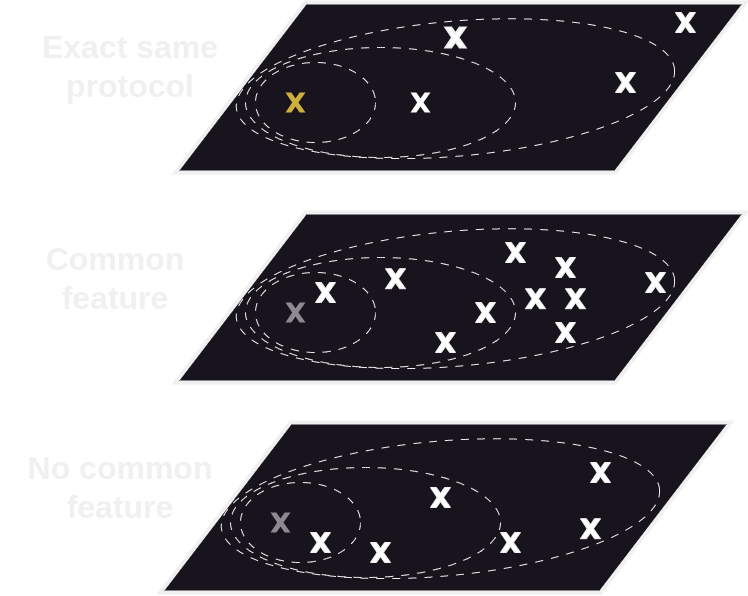
\includegraphics[scale=.26]{resources/dimensions.png}
    		\end{center}
	\end{column}

\end{columns}
\end{frame}

\begin{frame}
\frametitle{Routing Table Multi-Features Peers Selection}
\begin{columns}[onlytextwidth]
	\begin{column}{0.49\textwidth}
	    		\begin{center}
        		
\includegraphics[scale=.35]{resources/1-plan-buckets.png}\\
        		\medskip
        		\textit{Kademlia keyspace 2D\\distance projection}
        		\end{center}
	\end{column}
	\begin{column}{0.49\textwidth}
    		\begin{center}
        		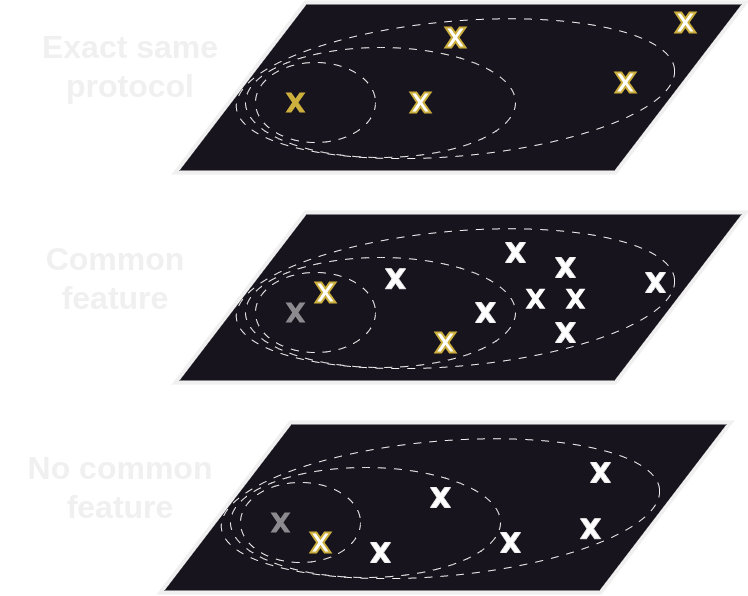
\includegraphics[scale=.26]{resources/dimensions-rt.png}
    		\end{center}
	\end{column}

\end{columns}
\end{frame}

\begin{frame}
\frametitle{Routing Table Multi-Features Peers Selection}
\begin{columns}[onlytextwidth]
	\begin{column}{0.49\textwidth}
	    		\begin{center}
        		
\includegraphics[scale=.35]{resources/1-plan-rt.png}\\
        		\medskip
        		\textit{Kademlia keyspace 2D\\distance projection}
        		\end{center}
	\end{column}
	\begin{column}{0.49\textwidth}
    		\begin{center}
        		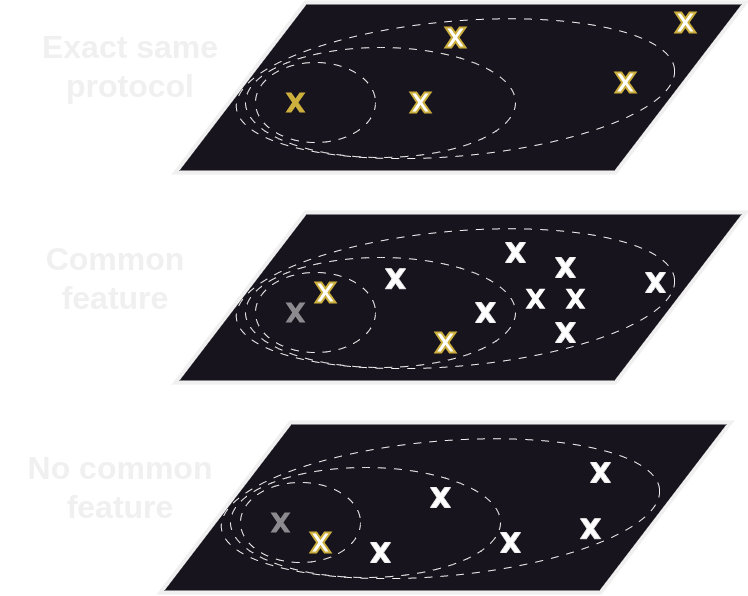
\includegraphics[scale=.26]{resources/dimensions-rt.png}
    		\end{center}
	\end{column}

\end{columns}
\end{frame}

\begin{frame}
\frametitle{Custom Routing Table Implementations}

\begin{columns}[onlytextwidth]
	\begin{column}{0.44\textwidth}
	    		\begin{center}
        		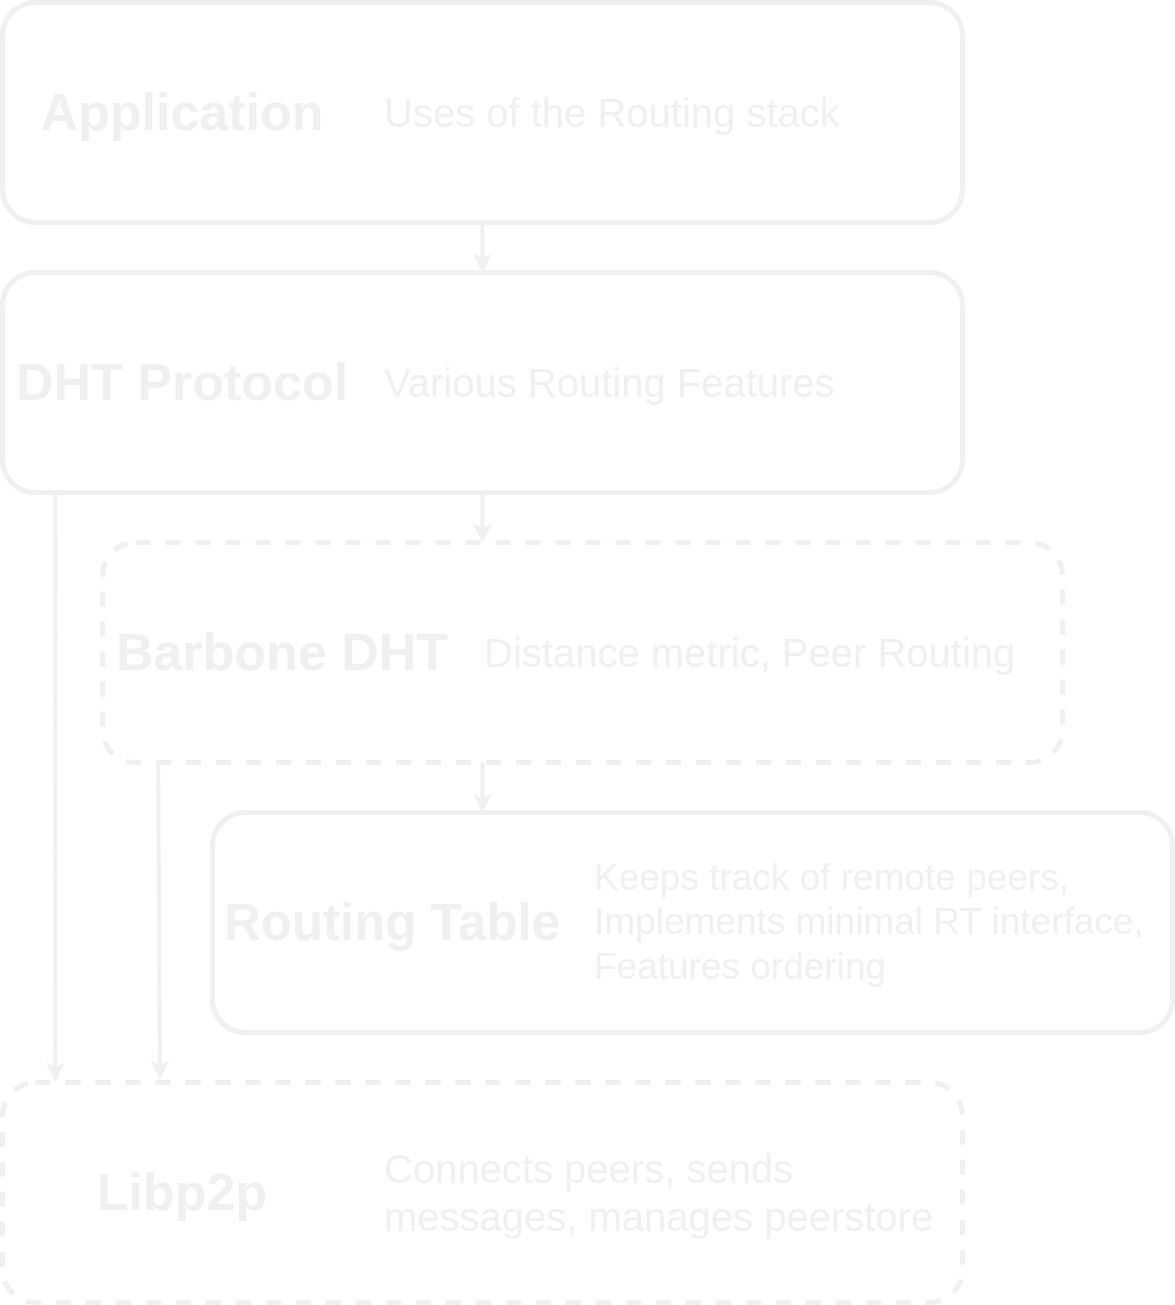
\includegraphics[scale=.14]{resources/composable-dht-stack.png}\\
        		\end{center}
	\end{column}
	\begin{column}{0.55\textwidth}
		\begin{itemize}
			\itemc Routing Tables can be tailored to fit applications special needs
			\itemc Must follow a simple interface with which the Barebone DHT will interact
			\bigskip
			\item[\greencube] Track remote peers' features
			\item[\greencube] Reachable peers in each bucket
			\item[\greencube] Implement \texttt{FindNClosest(key, feat)}
		\end{itemize}
	\end{column}

\end{columns}
\end{frame}

\begin{frame}
\frametitle{Example: IPFS Provide Operation}

\begin{columns}[onlytextwidth]
	\begin{column}{0.44\textwidth}
	    		\begin{center}
        		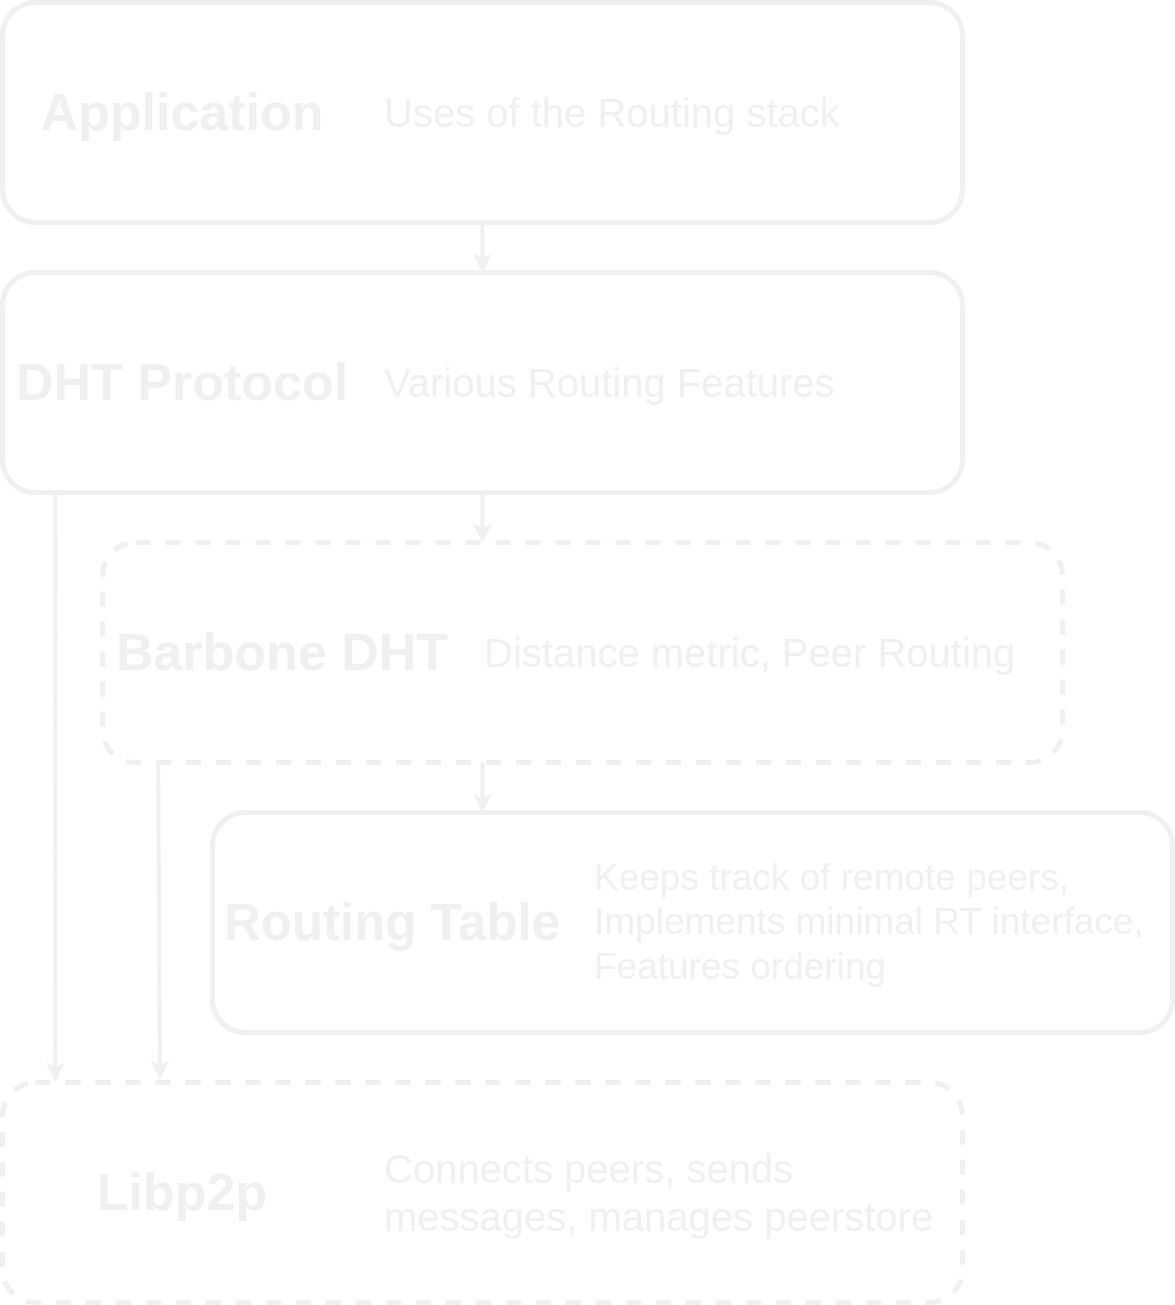
\includegraphics[scale=.14]{resources/composable-dht-stack.png}\\
        		\end{center}
	\end{column}
	\begin{column}{0.55\textwidth}
		\textit{Advertise to the DHT that I provide some content}
		\bigskip
		\begin{enumerate}
			\item IPFS Impl: asks DHT to provide CID
			\item Protocol DHT: find 20 closest peers to CID
			\item Barebone DHT: performs recursive query
			\item Protocol DHT: allocate Provider Record to the 20 closest peers
		\end{enumerate}
	\end{column}

\end{columns}
\end{frame}


\begin{frame}
\frametitle{Preventing Network Splits}
\begin{itemize}
	\itemc Record at least \texttt{N} peers supporting each feature in each bucket
	\begin{itemize}
		\item[\greencube] A remote peer can support multiple features
	\end{itemize}
	\itemc Decision free to the feature designer, but strongly recommended
	\itemc Worst case: the nodes running a common feature are split into multiple\\partitions, RPC routing won't work as expected
	\itemc Can be corrected with \texttt{FindFeature}
\end{itemize}
\end{frame}

\begin{frame}
\frametitle{\texttt{FindFeature} RPC}

\begin{itemize}
	\itemc Find other peers running a specific feature
	\itemc Can be implemented as a feature
	\itemc Upon receiving such a request, a node will return records of peers supporting the requested feature
\end{itemize}
\end{frame}

\begin{frame}
\frametitle{Bootstrappers nodes}

\begin{itemize}
	\itemc Any bootstrapper node can be used to join the DHT
	\itemc If no provided peers support required features, use \texttt{FindFeature} RPC
	\itemc Each protocol can alos have its own bootstrap nodes
\end{itemize}
\end{frame}


\begin{frame}
\frametitle{Main Benefits}

\begin{itemize}
	\itemc Welcome more applications to the libp2p DHT
	\itemc DHT Protocol Agility
	\itemc DHT Protocol Interoperability
	\itemc Increased Security
	\itemc Clear distinction between IPFS and libp2p.
\end{itemize}
\end{frame}

\begin{frame}
\frametitle{Protocol Upgrade Process}

\begin{itemize}
	\itemc DHT Protocols are not timeproof
	\begin{itemize}
		\item[\greencube] New RPCs are added, old RPCs are dropped
		\item[\greencube] Basic peer routing should't change
	\end{itemize}
	\medskip
	\itemc Migration transition period
	\begin{itemize}
		\item[\greencube] New and old features are concurrently supported, before old RPC is dropped
		\item[\greencube] For content routing, content must be advertised using both RPCs
	\end{itemize}
\end{itemize}
\end{frame}

\begin{frame}
\frametitle{Protocol Interoperability}

\begin{itemize}
	\itemc Libp2p global connectivity + global routability
	\itemc Interoperability between multiple libp2p networks using a DHT
	\bigskip
	\item[\greencube] Example: Filecoin could use the DHT to advertise content without having to implement every IPFS DHT RPC.
	\item[\greencube] Example: Filecoin could have its own DHT protocol optimized for its use, a DHT client could connect to both IPFS and Filecoin DHTs seamlessly
	\item[\greencube] Example: DHT interoperability between Filecoin, Ethereum, Polkadot etc.
\end{itemize}
\end{frame}

\begin{frame}
\frametitle{Tradeoffs}

\begin{itemize} 
	\itemc Larger Routing Table
	\begin{itemize}
		\item[\greencube] Additional storage: $\mathcal{O}(log(n))$
		\item[\greencube] Refresh process more expensive: $\mathcal{O}(log(n))$
	\end{itemize}
	\itemc Lookup latency stays the same or even decreases in small clusters
	\itemc Same routing guarantees in the sub-DHTs as in the current DHT
	\itemc Increased security: sybil attacks are more expensive in large networks
\end{itemize}
\end{frame}

\begin{frame}
\frametitle{Minimal requirements}

\begin{itemize}
	\itemc Libp2p
	\itemc \texttt{PeerID}s
	\itemc Standardized Peer Records
	\itemc Unified Feature Namespace
\end{itemize}
\end{frame}

\begin{frame}
\frametitle{Conclusion}

\begin{columns}[onlytextwidth]
	\begin{column}{0.69\textwidth}
	\begin{itemize}
		\itemc Enables other Libp2p apps to use the DHT
		\itemc Brings DHT Protocol Agility \& Interoperability
		\itemc Changes the Routing Table Selection Process
		\itemc Introduces new DHT RPCs as \textit{Features}
		\itemc Draws a clear line between IPFS and Libp2p in the DHT
	\end{itemize}
	\end{column}
	\begin{column}{0.29\textwidth}
		\begin{center}
			\qrcode[height=3cm]{https://www.notion.so/pl-strflt/Composable-DHT-Design-704a1d9ccfdd40d8977f08b7258f6f3c}\\
			\smallskip
			\textit{Composable DHT Notion Document (WIP)}
		\end{center}
	\end{column}
\end{columns}
\end{frame}


\begin{frame}
\frametitle{Q\&A}

\begin{columns}[onlytextwidth]
	\begin{column}{0.69\textwidth}
	\begin{itemize}
		\itemc All feedback is welcome
		\itemc Reach out in \texttt{\#probe-lab} on Filecoin Slack
	\end{itemize}
	\vspace{1cm}
	\begin{columns}[onlytextwidth]
	\begin{column}{.2\textwidth}
		\tikz\node [circle, minimum width = \linewidth,
			path picture = {
      			\node [] at (path picture bounding box.center) {
        				
\includegraphics[width=\linewidth]{../resources/avatar.jpg}
        			};
    		}] {};
	\end{column}
	\begin{column}{.78\textwidth}
		{\Large Gui Michel (@guissou)}
	\end{column}
	\end{columns}
	\end{column}
	\begin{column}{0.29\textwidth}
		\begin{center}
			\qrcode[height=3cm]{https://filecoin.io/slack}\\
			\smallskip
			\textit{Filecoin Slack}\\
		\end{center}
	\end{column}
\end{columns}

\end{frame}

\end{document}